\section{Microbenchmarks}
\label{sec:microbenchmarks}
In this section, we show the efficacy of our solutions through a set of microbenchmarks for 2 cases: data movement for data coupling nodes and data movement between compute nodes and I/O.

\subsection{Efficacy of proxies and pipeline technique}

%On BG/Q, we tested the system with 16 cores per node all communicate with 16 cores on another node, they transferred in all same links, resulting in 1.7GB/s at most. Due to the symmetry of mapping, it's more likely to all cores belonging to a nodes to connect with all cores belonging another nodes than connect with cores at different nodes. With 20 links per nodes, using multiple paths for data movement on BG/Q can results in significant throughput improvement. 

In this microbenchmark, we transfer data between two nodes through an intermediate nodes using pipelining and compare results with transferring data without using pipeline and with a direct transfer (default) scheme. We varied the data size from 1K  to 128MB.

\begin{figure}[!htb]
\centering
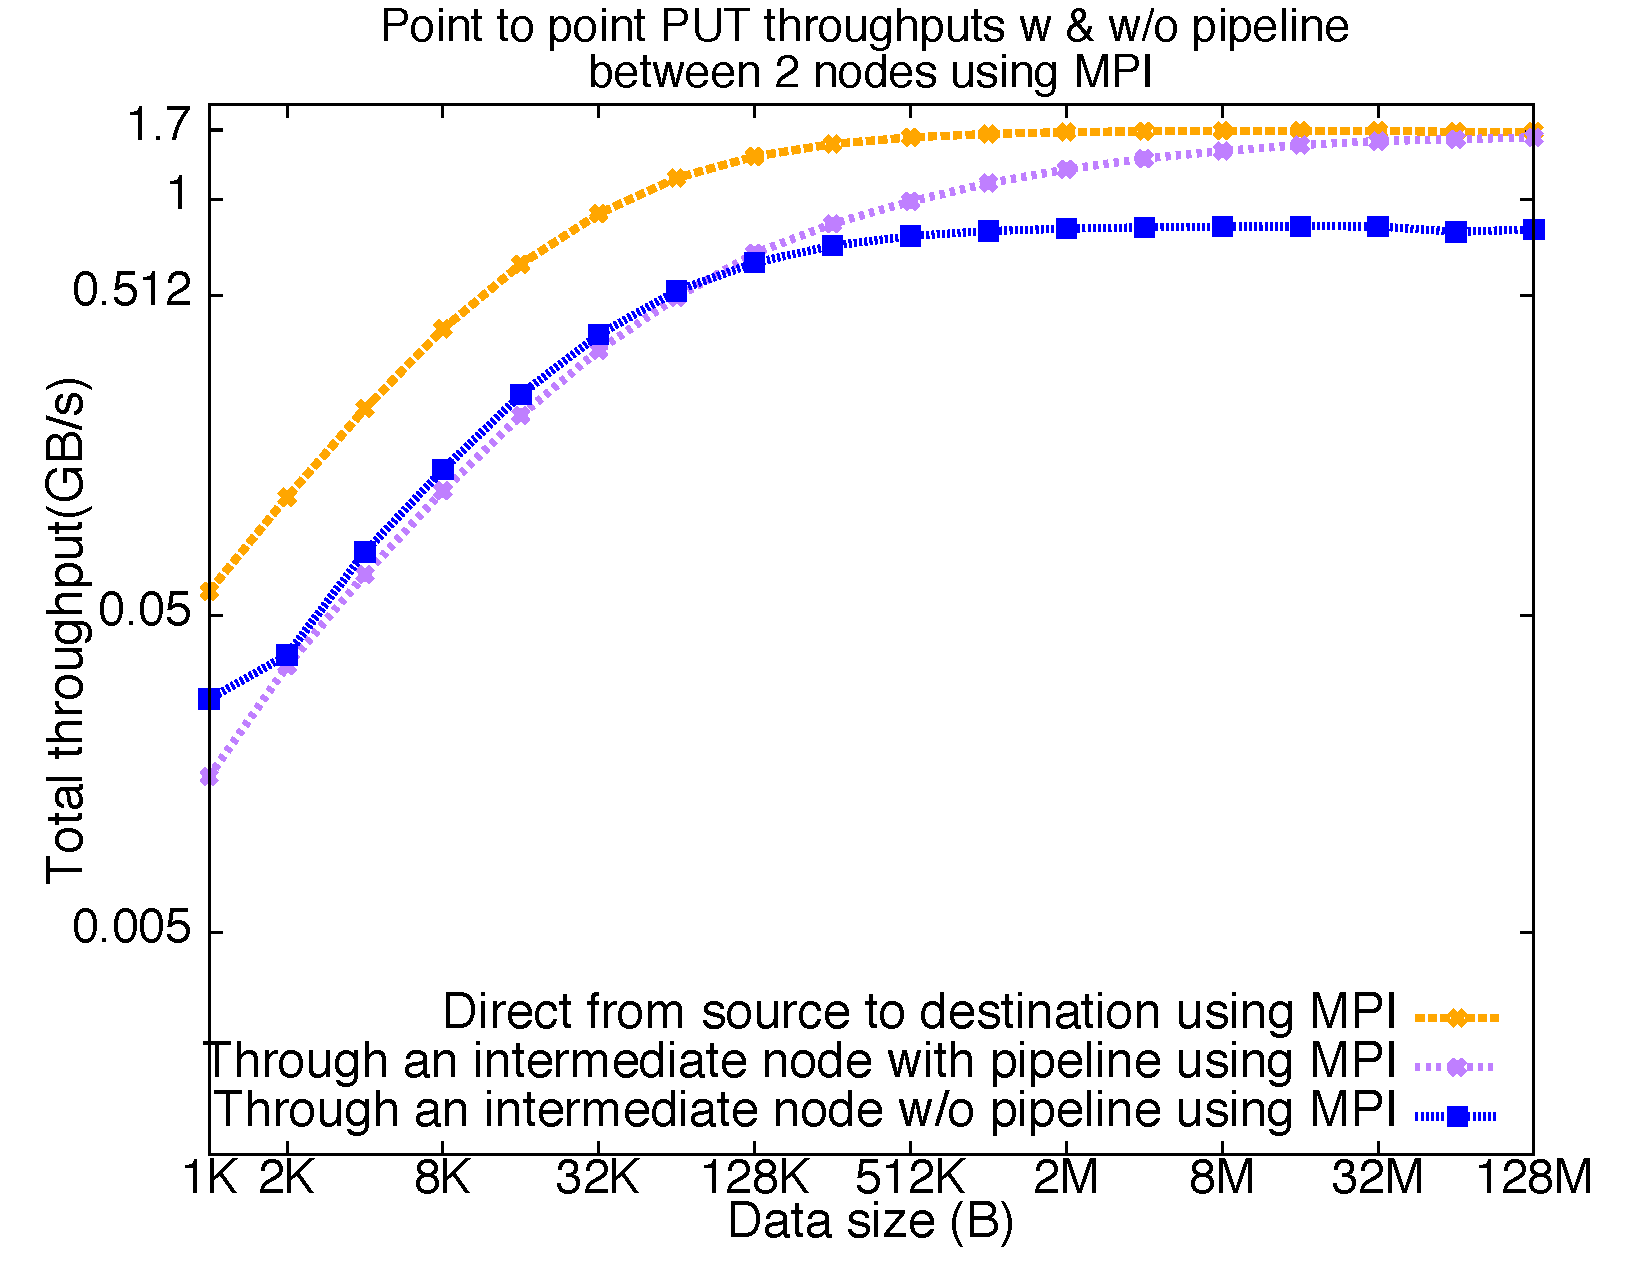
\includegraphics[scale=0.3]{figures/pipeline_mpi.pdf}
\caption{Using pipelining technique to mitigate the waiting time at proxy nodes}
\label{fig:pipeline_mpi}
\end{figure}

Fig. \ref{fig:pipeline_mpi} shows that transferring data through a proxy without using pipelining results a 50\% hit in performance over a direct transfer. This is because the proxy needs to wait until entire data is ready before forwarding it to the destination. By using pipelining, for message less than 64KB,  pipelining does not improve performance, however, for a message size larger than 64KB, pipelining demonstrates an improve performance. At a  message size of 1MB, 2MB, and 4MB, we achieve 70\%, 80\%, and  90\% respectively of the direct transfer bandwidth, and with larger size messages, we achieved a similar performance. Thus, with large size messages, pipelining technique can be used to transfer data through proxies. However, with small size messages, the performance gained is insignificant. Much of the performance overhead is due to the underlying rendezvous protocol design in MPI on the BG/Q. Next, we use PAMI to improve the performance for small messages. The next subsection, we show the efficacy of using PAMI on transferring small size messages.

\subsection{Quantifying computation used for data movement at proxies}
In this section, we quantify the time spent by the CPU for data movement, and we show that it is so small that it has no effect on the total time.

\subsection{Data movement for data coupling nodes}
In this benchmark, we show feasibility of the approach using proxies to increase transfer throughput between 2 compute nodes. We choose the first and the last node of a partition of 128 compute nodes with 2x2x4x4x2 torus. As the partition is large enough we are able to choose 4 proxies to transfer data in 4 directions +B, +C, +D, +E . In each node, only one MPI rank is used (when we use multiple MPI ranks per node to send data to the same destination, they all take the same output link, thus using one MPI rank is still valid and making the experiment easier). The data is transferred in increasing size from 1KB up to 128MB of data, with the size doubled each time. We use MPI\_Put to transfer data from source node to proxy nodes and then from proxy nodes to destination node. Each transfer is repeated multiple times with different data to eliminate any cache effect and achieve stable performance. The average transfer throughput between 2 nodes is reported in Figure \ref{fig:4proxies}.

\begin{figure}[!htb]
\vspace{-0.1in}
\centering
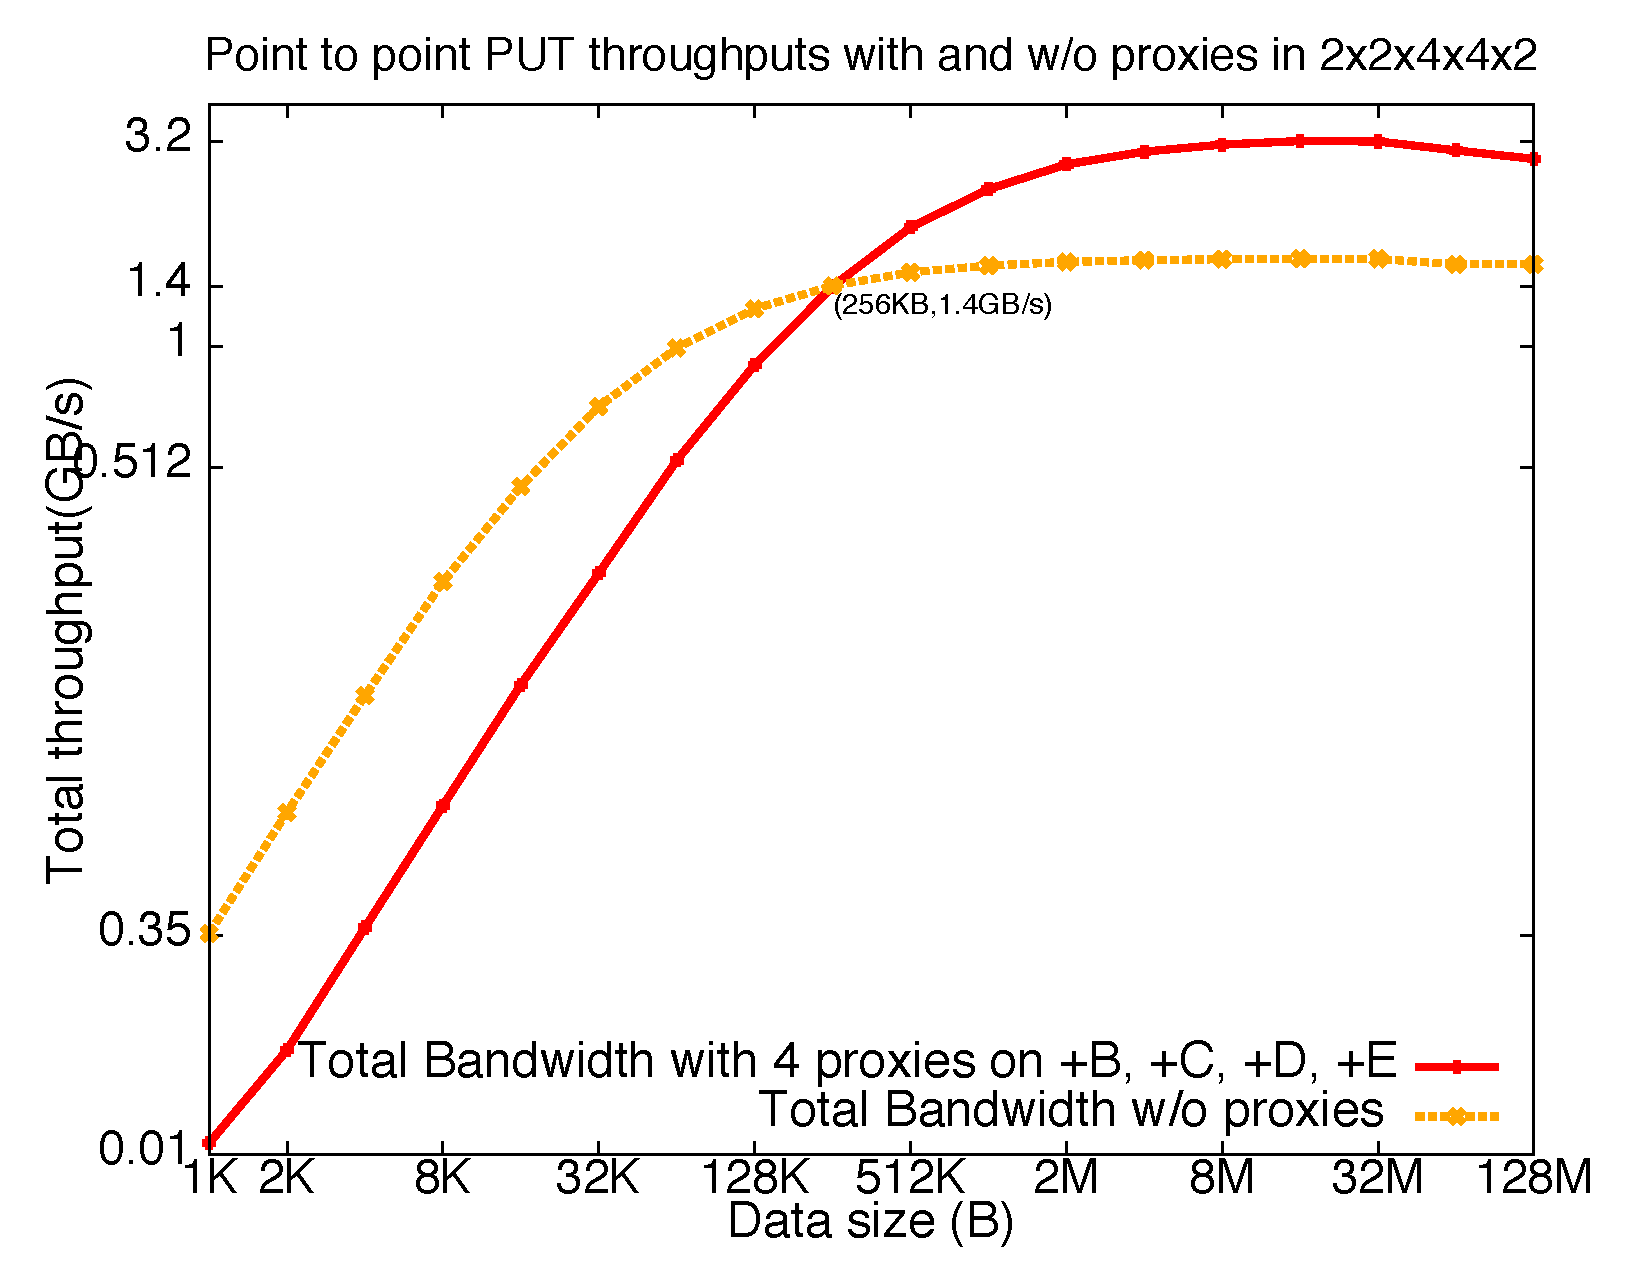
\includegraphics[scale=0.3]{figures/4proxies}
\vspace{-0.2in}
\caption{Using 4 proxies to improve data transfer throughput between 2 nodes}
\vspace{-0.1in}
\label{fig:4proxies}
\end{figure}

As the figure shows, for the small messages, direct transfer yields better performance. With large message, proxy-based transfers outruns direct transfer with $2\times$ better performance. This is foreseen with the reasons we mentioned before: with small messages, extra time caused by injecting and copying messages is significantly larger than the transferring time. It happens in the opposite way with large messages. The message size threshold to switch from direction transfer to proxy-based transfer is 256KB, yielding 1.4GB/s per link. After the threshold, direct transfer slowly reaches to maximum ~1.6BG/s while proxy-based transfer continue to thrive until ~3.2GB/s. Thus, the benchmark shows that proxy-based approach is feasible and can result significant improvement.

As data movement in multiphysics applications is done by more than 2 single nodes, the second benchmark elucidates the feasibility and achievable throughput for data movement between two groups of nodes. In this experiment, we transfer data between two groups of nodes, wherein each group has 256 nodes in a 4x4x4x16x2 torus of a 2K nodes partition. One group is at one corner of the partition, the other one is at the other end of the partition. The data size is also from 1KB to 128MB with doubled size each step. The experiment is repeated for a number of times. We are able to choose 3 proxies for each node. The Figure \ref{fig:3groxies} shows the average throughput measured.

\begin{figure}[!htb]
\vspace{-0.1in}
\centering
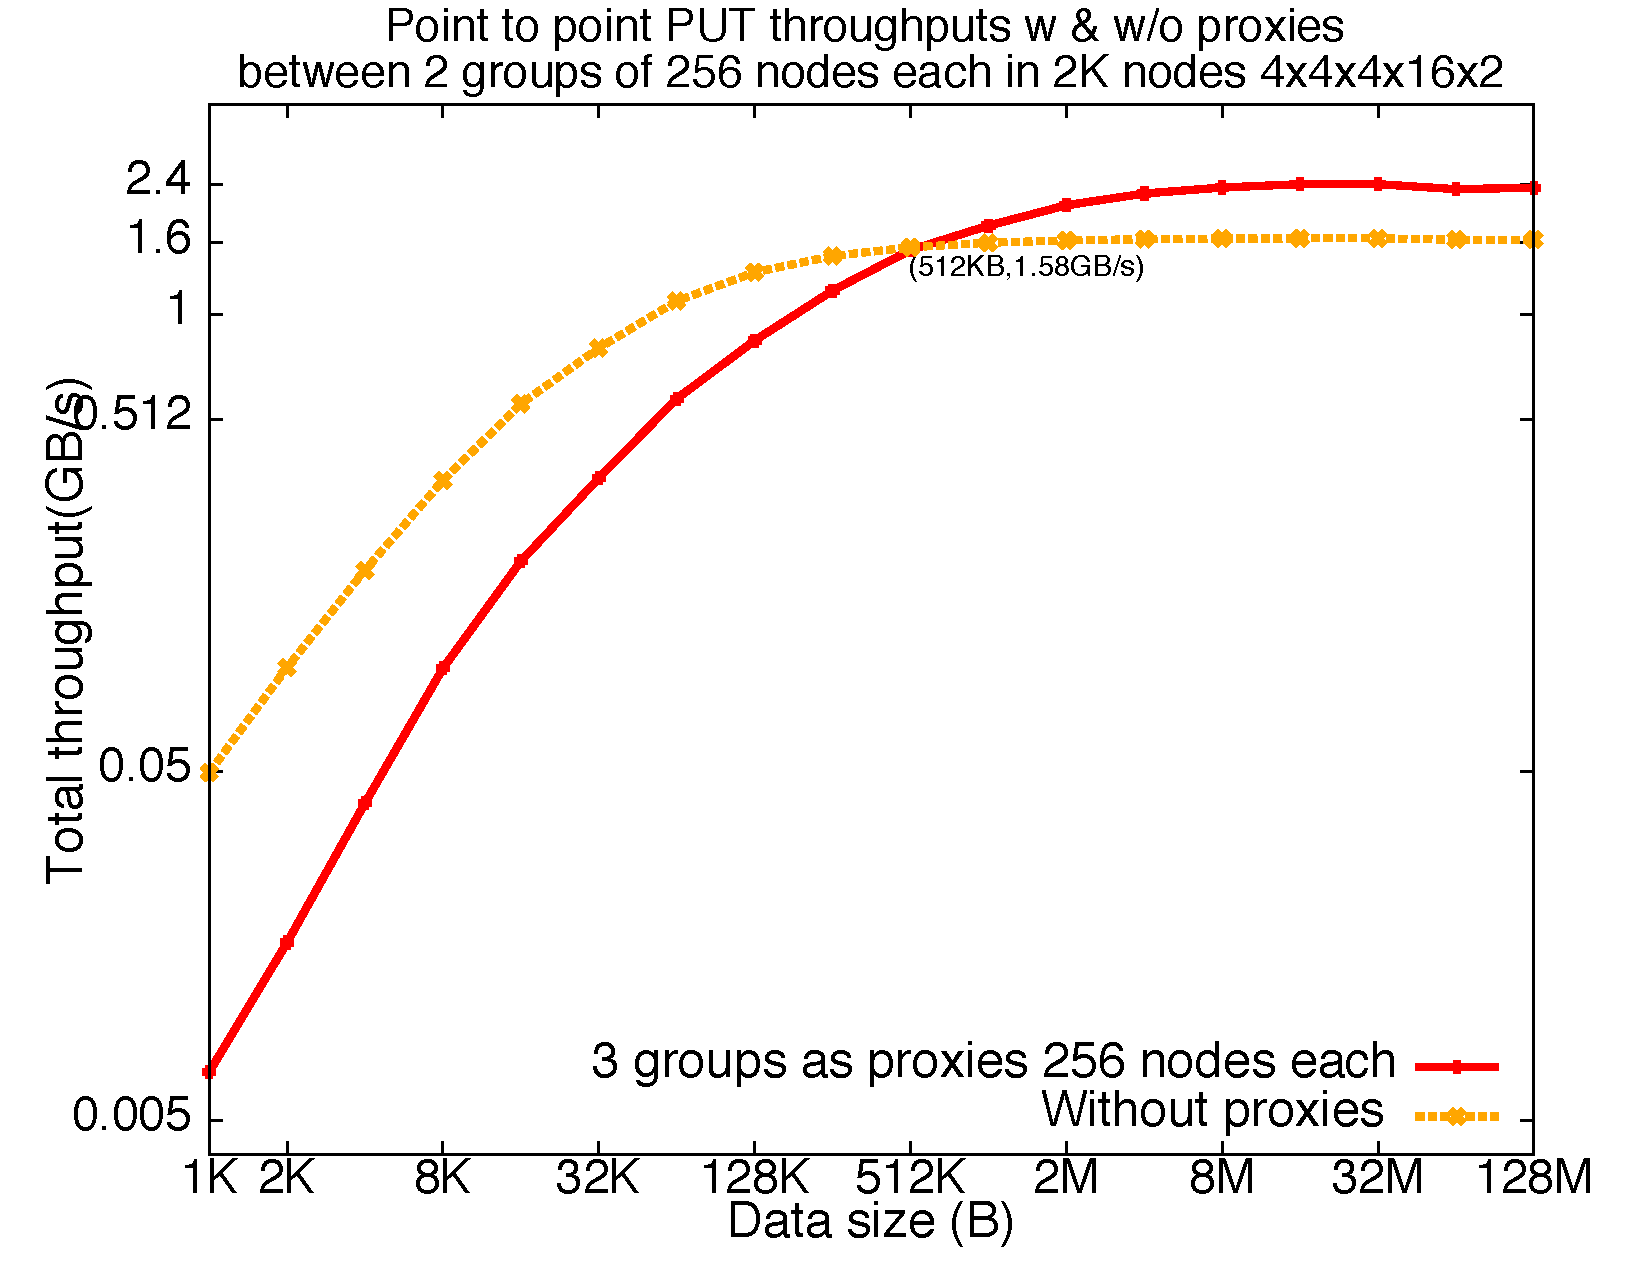
\includegraphics[scale=0.3]{figures/3groxies}
\vspace{-0.2in}
\caption{Using 3 group of proxies to improve data transfer bandwidth between 2 group of nodes}
\vspace{-0.1in}
\label{fig:3groxies}
\end{figure}

In the figure, we once again see that with small messages, direct transfer is better than proxy-based transfer. The threshold for this case increases to 512KB. At that message size, direct transfer also reaches to its maximum throughput, while the proxy-based transfer still has big room to increase up to 2.4GB/s. The performance increases $1.5\times$ as predicted since 3 proxies are used for each nodes. This benchmark shows that proxy-based data transfer is feasible for data transfer between groups of nodes. And we can achieve significant improvement in certain cases.

As we have mentioned in Section \ref{sec:approaches}, we need at least k $>$ 2 proxies per each data transfer to benefit from proxies. The more proxies we can use the better performance we can gain. However, as the size of communicating groups increases, the number of proxies we can set up decreases. If we add more proxies beyond the maximum possible proxies, data movements by extra proxies intervene existing ones and eventually degrade overall performance. The Figure \ref{fig:num_groxies} demonstrates the situation.

\begin{figure}[!htb]
\vspace{-0.1in}
\centering
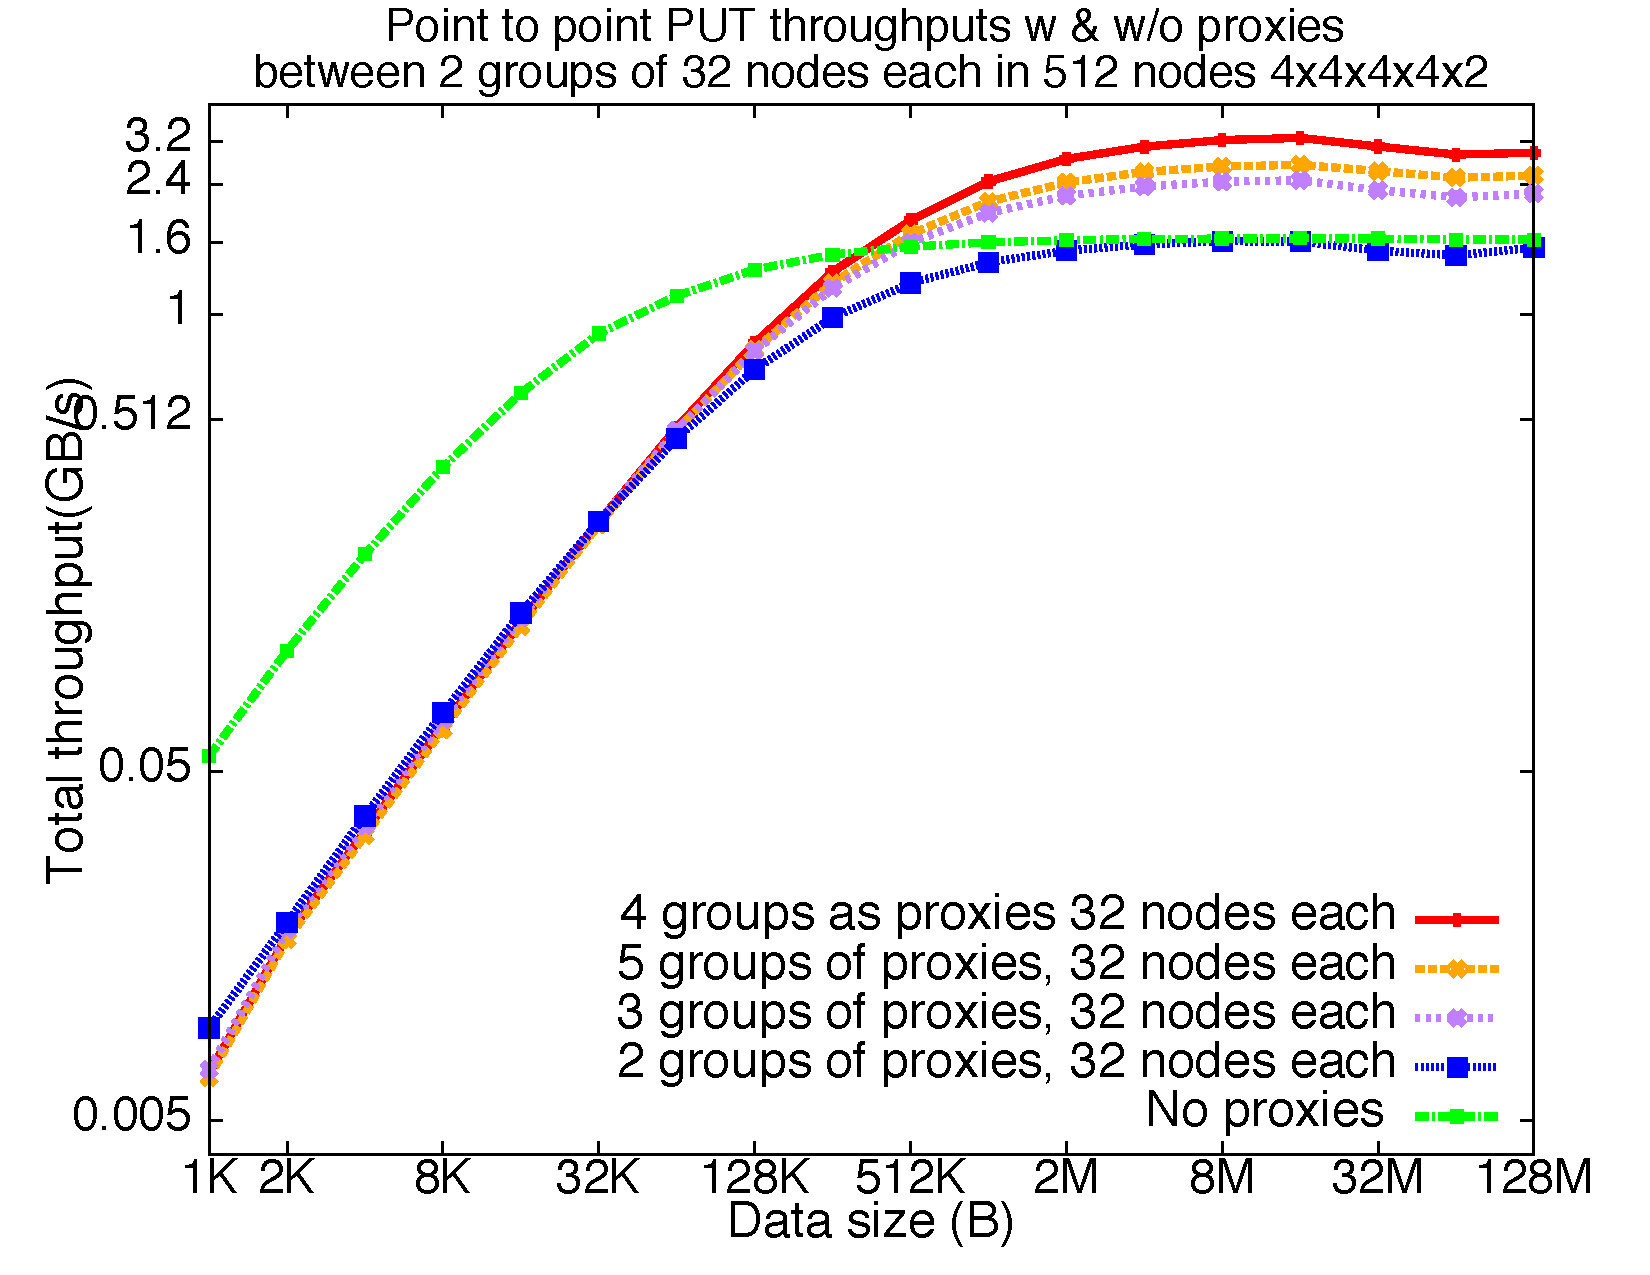
\includegraphics[scale=0.3]{figures/num_groxies}
\vspace{-0.2in}
\caption{Performance variance with number of proxies}
\label{fig:num_groxies}
\vspace{-0.1in}
\end{figure}

With the torus 4x4x4x4x2 and 2 groups of 32 nodes each, we can set up at most 4 groups of proxies along A+, A-, B+, B- dimensions. The 5th proxy is the source node itself. As Figure \ref{fig:num_groxies} shows, when we increases the number groups of proxies from 2 to 3 and to 4, the throughput increases from no-improvement, to 1.5$\times$ and to 2$\times$. Thus, with large message sizes, we can gain k/2 times performance with k being the number of proxies. However, when we increase number of proxies to 5, the performance starts to drop due to intervention among concurrent data movements. Therefore, choosing number of proxies together with their locations is important to maximize throughput.

The above three benchmarks demonstrate the efficaty of our solutions for data movement between compute nodes. In the next subsection, we evaluate our approaches in the case of data movement between compute nodes and I/O nodes. 

%\subsection{Sparse data patterns}


%In the next subsection, we present our benchmarks on the two data patterns generated.
%\subsection{Staging}

\subsection{Data Movement to I/O nodes}
We perform a weak scaling study with two sparse data patterns, and scale the number of cores from 2,048 to 131,072 cores on the Mira BG/Q system. 

\begin{itemize}
\item Pattern 1: Uniform distribution data where data size of a MPI rank is uniformly distributed between 0 and 8MB.  Data is generated by using \textit{srand()} and \textit{rand()} functions in C/C++ and using \textit{time(NULL)} as a seed.  Total data size is about 50\% of the dense data. The distribution of the data size is shown in Figure \ref{fig:uniform}.
\item Pattern 2: Pareto distribution data where many of MPI ranks have data size of 0 bytes or very low size, and a few of MPI ranks have data size of 8MB or close by. The total data size is about 20\% of the dense pattern. The distribution of the data is shown in Figure \ref{fig:pareto}
\end{itemize}

In the data pattern 1, data sizes are uniformly distributed among nodes. This data pattern can be seen when we want to analyze data from different regions with different resolutions. Depending on the resolution, data sizes may vary accordingly.

\begin{figure}[!htb]
\vspace{-0.2in}
\centering
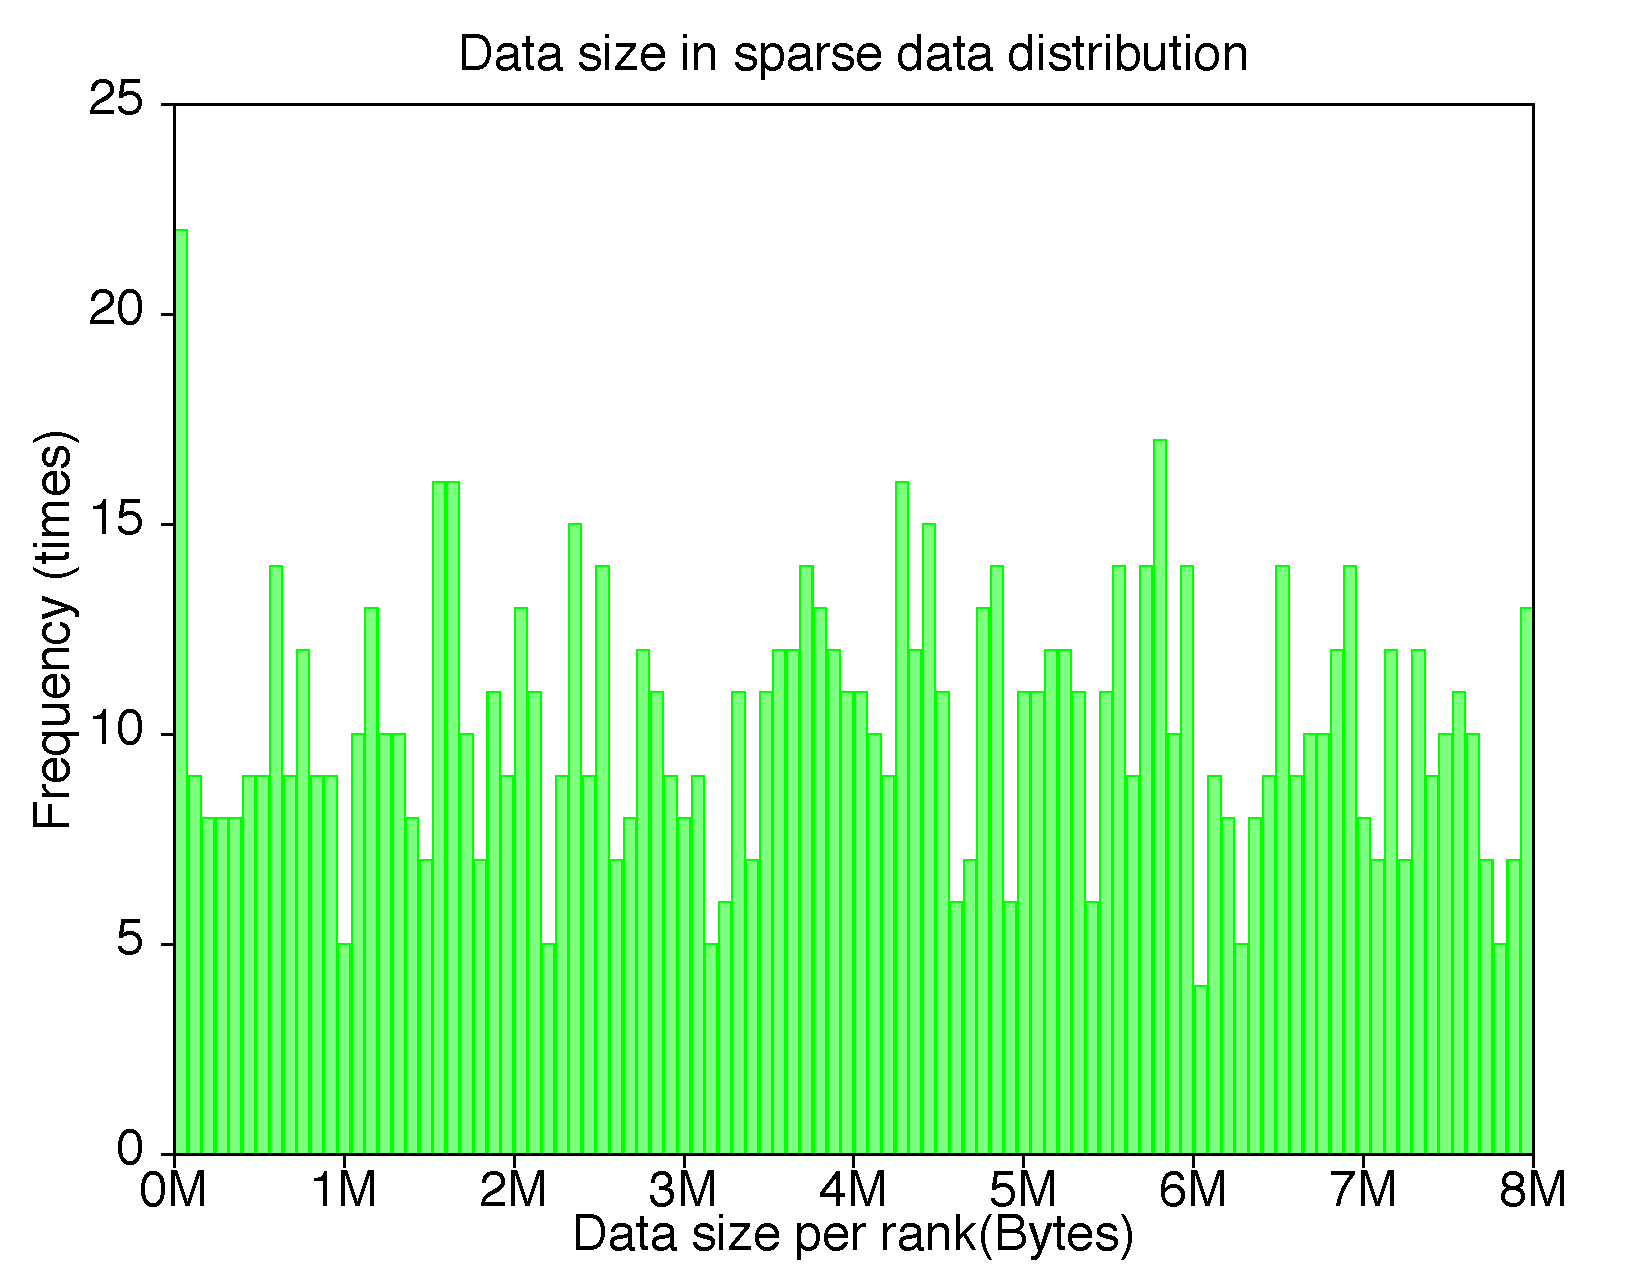
\includegraphics[scale=0.3]{figures/uniform.pdf}
\caption{Pattern 1: Histogram of data sizes for 1,024 processes using time(NULL) function with size from 0 to 8MB}
\label{fig:uniform}
\vspace{-0.1in}
\end{figure}

On the other hand, the data pattern 2 represents the case where data are sparse but not uniformly distributed. There are many nodes with almost no data while some nodes have large volume of data. This data pattern happens where we want to write out data from a region of contiguous MPI ranks while ignoring other regions.

\begin{figure}[!htb]
\vspace{-0.1in}
\centering
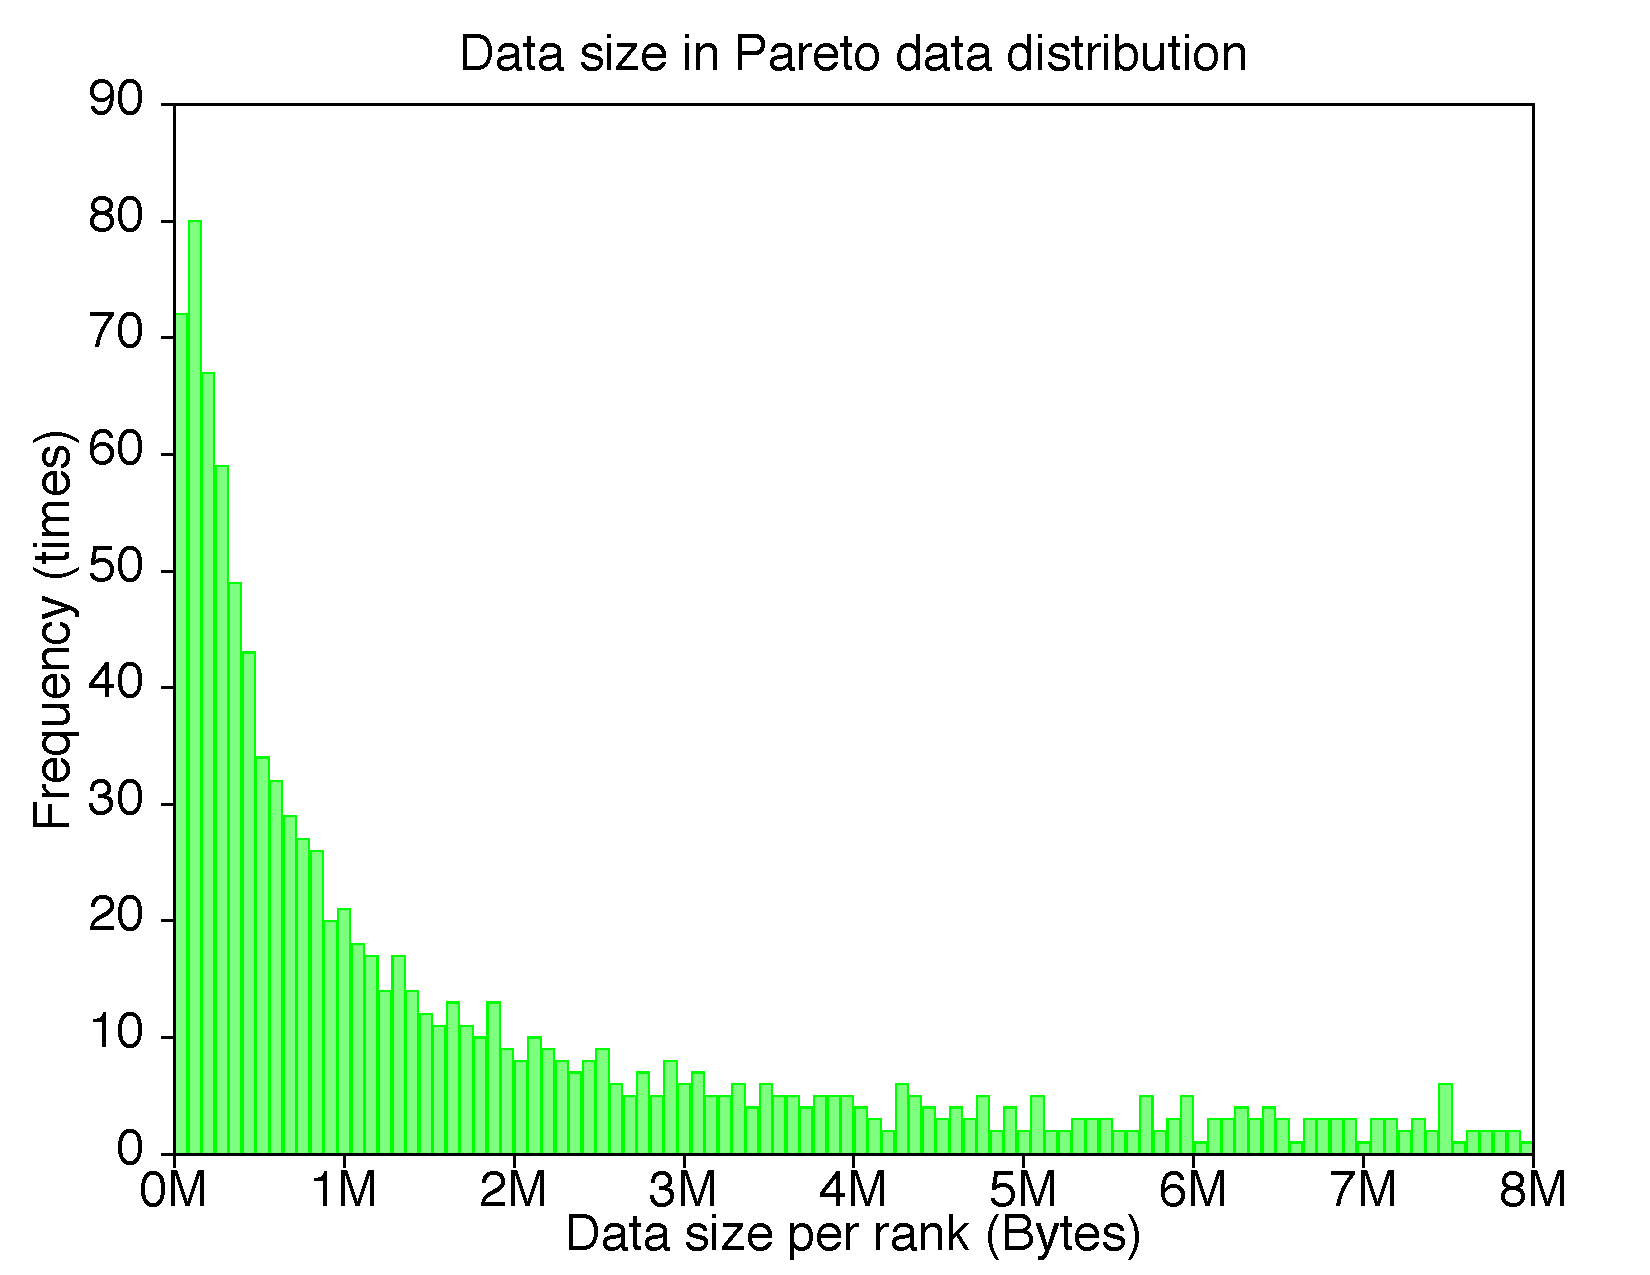
\includegraphics[scale=0.3]{figures/pareto.pdf}
\vspace{-0.1in}
\caption{Pattern 2: Histogram of data sizes of 1,024 processes using Pareto distribution function with size from 0B to 8MB}
\label{fig:pareto}
\vspace{-0.1in}
\end{figure}

On data pattern 1, we write roughly 8GB at 2,048 cores and 274GB of data at 131,072 cores. On data pattern 2, we write 3.4GB at 2,048 cores to 119GB of data at 131,072 cores. We compare the performance of performing aggregation for 2 data patterns using our approach and default MPI Collective I/O.

\begin{figure}[!htb]
\vspace{-0.1in}
\centering
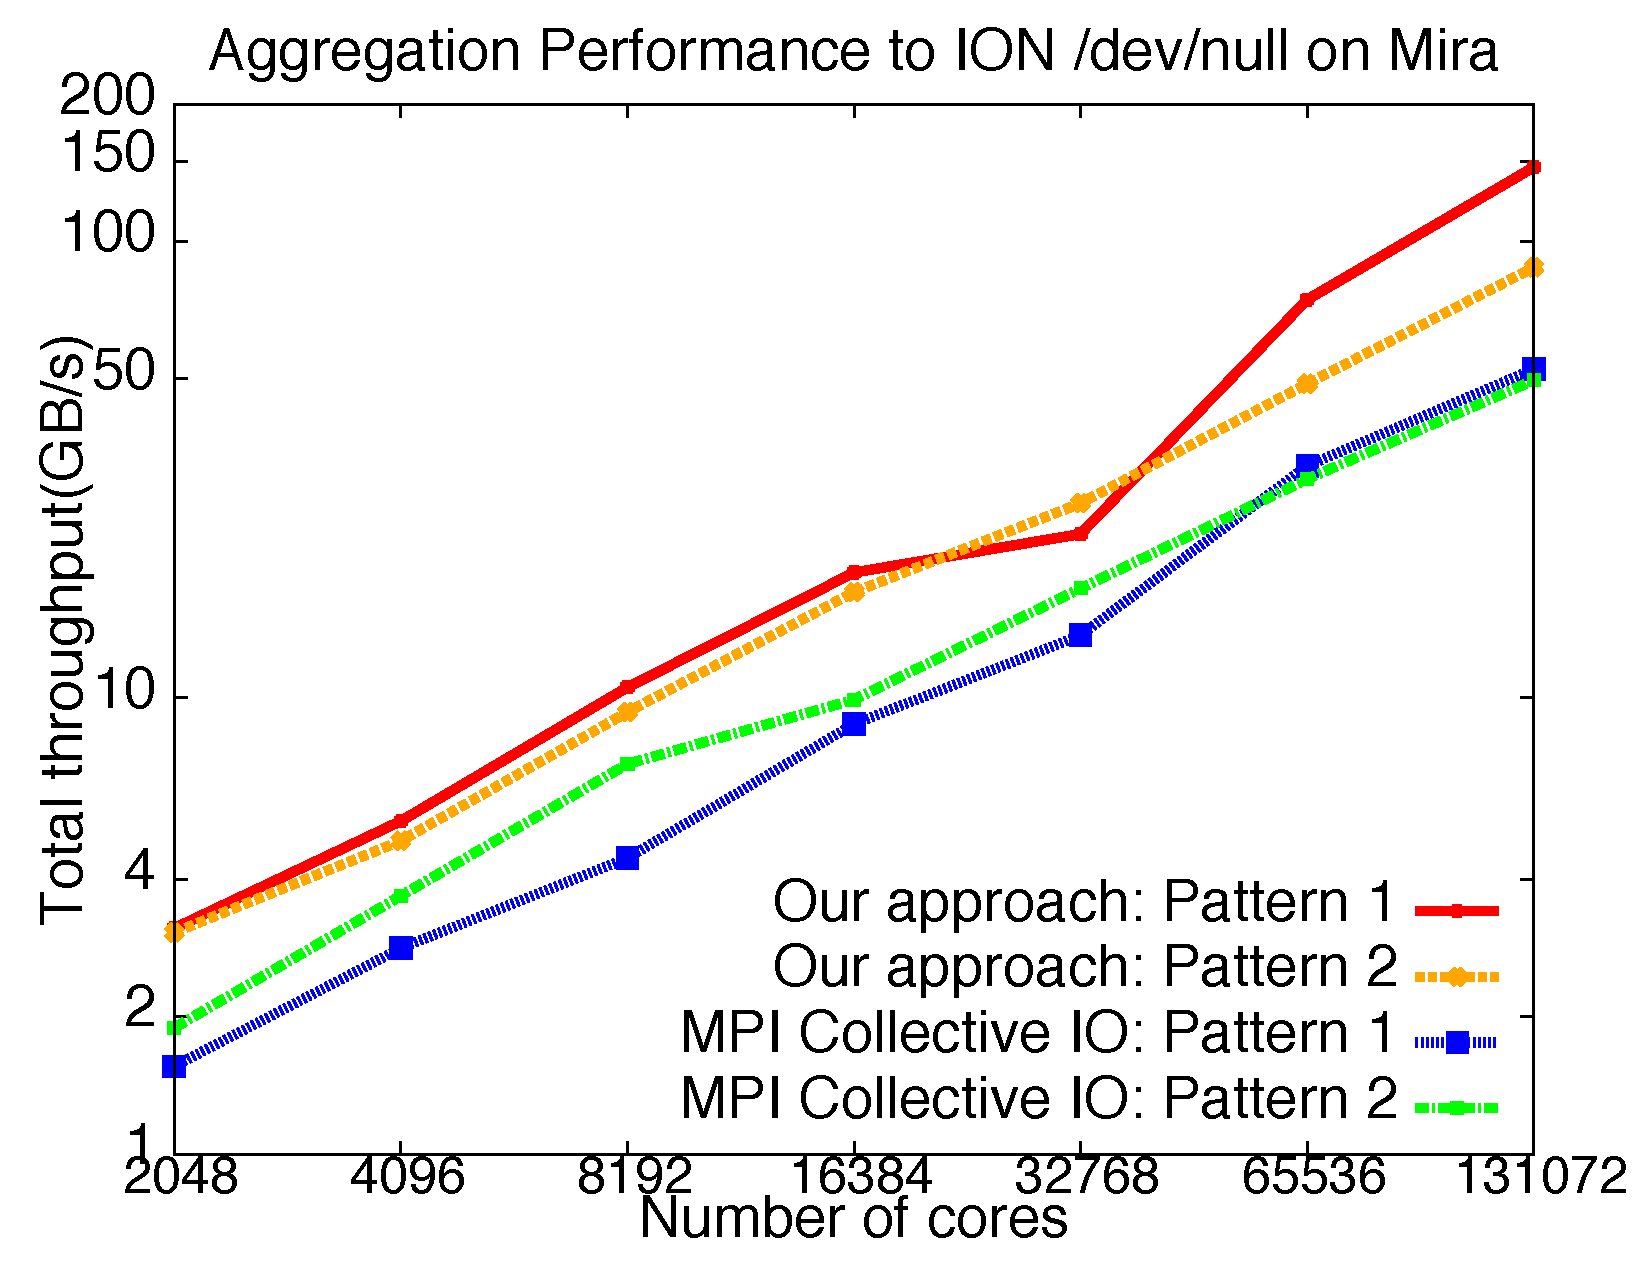
\includegraphics[scale=0.3]{figures/mira_agg.pdf}
\vspace{-0.2in}
\caption{Aggregation throughputs on Mira}
\vspace{-0.2in}
\label{fig:mira_agg}
\end{figure}

Figure \ref{fig:mira_agg} depicts the performance of our topology-aware multipath data movement approach in comparison to the default MPI-I/O for the two sparse data patterns as we scale from 2,048 cores to 131,072 cores on the Mira BG/Q system. On the data pattern 1 (uniformly distributed data), we observe  $2\times$ improvement at 2,048 cores. The performance increases as we scale and we achieve up to $3\times$ at 131,072 cores. On the data pattern 2 (pareto distributed data), we gain $1.5\times$ improvement at 2,048 cores and $2\times$ improvement at 131,072 cores. Thus, we observe that leveraging network interconnect topology and multipaths plays an important role at small scale and is critical at large scale. With the increased use of in-situ analysis for supercomputing,  sparse data patterns for I/O are becoming increasingly important and our approaches help provide more insights for improved performance.